\documentclass[times, 10pt,twocolumn]{article} 
\usepackage{latex8}
\usepackage{times}
\usepackage{url,hyperref}
\usepackage{subfigure}
\usepackage{tikz}
\usepackage{examplep}
\usepackage{moreverb}
\usepackage{algorithm}
\usepackage{boxedminipage}
\usepackage[noend]{algpseudocode}
\usepackage{listings}
\usepackage{amsmath,amsfonts,latexsym,graphicx}
\lstset{language=C,numbers=left,basicstyle=\footnotesize,numberstyle=\footnotesize}
\usetikzlibrary{arrows,decorations.pathmorphing,backgrounds,fit,shapes.geometric}
\usepgflibrary{shapes.geometric}


%\documentclass[11pt]{article}
%\usepackage{fullpage}
%\usepackage{ijcai09}


%\setlength{\oddsidemargin}{0in}
%\setlength{\topmargin}{0in}
%\setlength{\textwidth}{6.5in}
%\setlength{\textheight}{8.5in}

\newtheorem{fact}{Fact}[section]
\newtheorem{lemma}{Lemma}[section]
\newtheorem{theorem}[lemma]{Theorem}
\newtheorem{assumption}[lemma]{Assumption}
\newtheorem{definition}[lemma]{Definition}
\newtheorem{corollary}[lemma]{Corollary}
\newtheorem{prop}[lemma]{Proposition}
\newtheorem{claim}[lemma]{Claim}
\newtheorem{remark}[lemma]{Remark}
\newtheorem{prob}{Problem}
\newtheorem{conjecture}{Conjecture}


\newenvironment{mylisting}
{\begin{list}{}{\setlength{\leftmargin}{1em}}\item\scriptsize}
{\end{list}}

\newenvironment{mytinylisting}
{\begin{list}{}{\setlength{\leftmargin}{1em}}\item\scriptsize\texttt}
{\end{list}}
\newenvironment{proof}{\vspace{-0.15in}\noindent{\bf Proof:}}%
        {\hspace*{\fill}$\Box$\par}
\newenvironment{proofsketch}{\noindent{\bf Proof Sketch.}}%
        {\hspace*{\fill}$\Box$\par\vspace{4mm}}
\newenvironment{proofof}[1]{\smallskip\noindent{\bf Proof of #1.}}%
        {\hspace*{\fill}$\Box$\par}

\newcommand{\etal}{{\em et al.}\ }
\newcommand{\assign}{\leftarrow}
\newcommand{\eps}{\epsilon}
%\documentstyle[times,art10,twocolumn,latex8]{article}

%------------------------------------------------------------------------- 
% take the % away on next line to produce the final camera-ready version 
\pagestyle{empty}

%------------------------------------------------------------------------- 
\begin{document}

\title{Parallel Information Set Generation for Kriegspiel 
       }

\author{Mark Richards, Abhishek Gupta, Osman Sarood and Laxmikant V. Kale\\
Department of Computer Science\\ 
University of Illinois\\ 
Urbana, IL\\ {mdrichar, gupta59, sarood1, kale}@illinois.edu\\
% For a paper whose authors are all at the same institution, 
% omit the following lines up until the closing ``}''.
% Additional authors and addresses can be added with ``\and'', 
% just like the second author.
%\and
%Second Author\\
%Institution2\\
%First line of institution2 address\\ Second line of institution2 address\\ 
%SecondAuthor@institution2.com\\
}

\maketitle
\thispagestyle{empty}

%\newtheorem{lemma}{Lemma}
%\newtheorem{theorem}[lemma]{Theorem}
%\begin{document}

%\title{Information Set Generation in Kriegspiel}
%\author{Abhishek Gupta\qquad Mark Richards\qquad Osman Sarood\\University of Illinois at Urbana-Champaign\\CS598LVK:
%Parallel Combinatorial Search} \maketitle

\begin{abstract}
Information Set Generation is the identification of the set of paths in an imperfect information game tree that are
consistent with a player's observations.  The ability to reason about the possible game history is critical to the
performance of game playing agents.  ISG represent a class of combinatorial search problems which is computationaly intensive but difficult to efficiently parallelize.

In this paper, we address the parallelization of information set generation in the context
of Kriegspiel (partially observable chess).  We implement the algorithm on top of a general purpose combinatorial search
engine and discuss its performance under different load balancing strategies and with different grain-size parameters.
We achieve speedups of over 500 on 1024 processors, far exceeding previous scalability results for game tree search applications.
\end{abstract}

\Section{Introduction}
In imperfect information games, players do not have access to full knowledge of
the world. Examples of imperfect information include hidden cards in
Poker~\cite{billings02challenge} or Bridge~\cite{ginsberg96partition}, hidden
tiles in Scrabble~\cite{richards07opponent}, or hidden pieces 
Kriegspiel (partially observable chess)~\cite{li94chess}. The game tree nodes
that are indistinguishable to a player because they differ only in the
information that is hidden to the player by rule compose that player's {\em
information set.}  The ability to estimate the value of the possible states and
to reason about the probability distribution over those states is crucial to
playing imperfect information games well~\cite{thielscher12hyperplay}. 

Information Set Generation (ISG) is an operation that game tree search agents
can use to identify nodes in the game tree that are consistent with their
observations~\cite{richards12reasoning}.  Because the operation is relatively
expensive and may be repeatedly applied by a decision-making agent, its
efficiency is a key factor in an agent's overall performance. Information set generation is not the same problem as solving a game tree, although it is arguably a necessary subroutine for quality game play in imperfect information games. 

The term {\em belief state} is sometimes used interchangeably with information set to refer to a probability
distribution over possible worlds.  The latter term comes from the game theory community and is preferred here.  A node
in a game tree denotes not only the current state of the game, but also uniquely defines a path from the initial state
or root node.  Thus, a game tree node implicitly encodes not only the current state of the game but also the complete
history of all decisions made by all players up to that point in the game, including the outcome of any chance moves
such as dice rolls or card shuffling.  Knowing one's information set means knowing all possible game histories.

For many specific games, solving the information set generation problem is trivial.  For example, in a poker game, it is easy to
see that the unseen cards held by a player's opponents may be any permutation of the cards not seen by that player
(i.e., hole cards and any revealed community cards).  After the betting rounds, it would not be reasonable to assume
that each of these permutations of unseen cards is equally probable, as betting decisions made by the players up to that
point would be affected by the quality of those players' cards.  But the set of {\em possible} hands for all of the
opponents is easy to conceive and enumerate.

In the game of Kriegspiel, information set generation is much more complicated.  The player knows the opponent's position with
certainty when the game begins, but after the initial move there may be varying levels of uncertainty about the location
of the opponent's pieces.  Unlike poker, it is not possible to simply permute all of the opponent's possible pieces over
all of the squares not occupied by the player's own pieces.  A configuration of pieces for the opponent is only valid if
it can be reached by a legal sequence of moves.  In the general case, finding the nodes in an information set is a
combinatorial search problem.

In this work, we show that ISG for Kriegspiel can be efficiently parallelized. The primary contributions of this work are the following. We describe an approach to efficient parallelization of an application which is not typical of high performance computing domain. We present scalability results for our parallel implementation of information set generation algorithm for the game of Kriegspiel using real game problem instances. Further, we demonstrate the effect of load balancing and grain size on parallel performance of our solution. 

The paper is organized as follows.  In Section~\ref{Background}, we review necessary background information, including the rules of kriegspiel and the nature of the information set generation problem.  In Section ~\ref{ParSSSE}, we describe the {\sc Charm++} Parallel State Space Search Engine (ParSSSE) platform.  We then provide our experimental results in Section~\ref{Results}.  Related work is discussed in Section~\ref{Related}.  We conclude with a discussion of future work.

%\Section{Information Set Generation}
\Section{Background: Kriegspiel}
Information Set Generation is a widely adopted operation used in game trees search. Here, we present our techniques and results in the context of a particular game - Kriegspiel. However, the techniques and framework presented in this paper is general and can be applied to other imperfect games for generating information set.
%\Section{Background: Kriegspiel}
Kriegspiel, or partially observable chess,  was invented by Henry Michael Temple in 1899.  Historically, the
game has required three parties: two competing players and one referee.  Today,
players often compete over a computer network, with the role of the referee
being automated.  One player sees and controls only the white pieces; the
other, black.  The referee track of both sets of pieces.  The players alternate
moves as in a regular chess game, but instead of openly declaring their moves,
they secretly communicate move requests to the referee.  The referee, who knows
the location of all pieces, checks the legality of the move.  

If the move is legal, the referee makes executes the move and announces that a
legal move has been made and that it is the other player's turn to move.  If
the move is illegal because it is blocked by an opponent's piece or would place
or leave the active player in check, the referee announces, ``No.''  The player
then continues, without penalty, to attempt moves until one finally succeeds.
If a player has no legal moves because of stalemate or checkmate, the referee
announces the game's result.

The referee makes other announcements besides declaring move illegal, and there
are several variations of the game that differ only in the nature of these
announcements.  All declarations by the referee are made to both players.  In
particular, a player will hear and know if her opponent has attempted an
illegal move, and will thus know that her opponent's pieces are configured in
such a way as to allow at least one attemptable move that is blocked or would
leave him in check.  

The referee announces when a player is in check. In the case of the capture,
the referee announces the location of the piece that was captured but not its
identity.  Because there is no penalty for making illegal moves, it is often to
a player's advantage to attempt to make moves which are likely to be illegal,
as hearing such declarations from the referee can provide important information
to a player about the location of the opponent's pieces.  In particular, since
a diagonal move by a pawn is legal only the case where such a move would
capture an opponent's piece, it could potentially be profitable to attempt all
or many pawn captures on every turn.  In order to speed the game up, the
referee declares, at the beginning of a player's turn, all locations where a
pawn capture is possible. 

In general, any move that is legal in a regular chess match may be at least
attempted by a player in Kriegspiel.  And any Kriegspiel move that is
ultimately allowed by the referee would also be a legal move in chess.    

%\SubSection{Example}
\begin{figure}[ht]
\centering
\begin{minipage}[b]{0.45\linewidth}
\centering
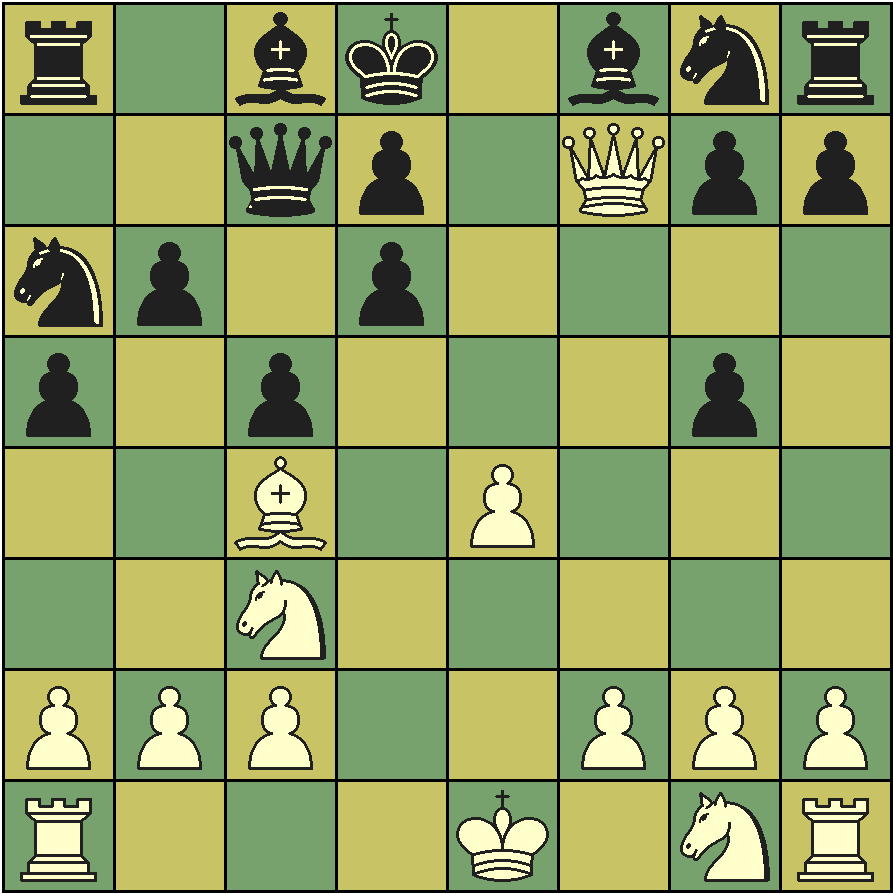
\includegraphics[width=0.7\textwidth]{images/9B.png}
\caption{Actual Position}
\label{fig:figure1}
\end{minipage}
\hspace{0.5cm}
\centering
\begin{minipage}[b]{0.45\linewidth}
\centering
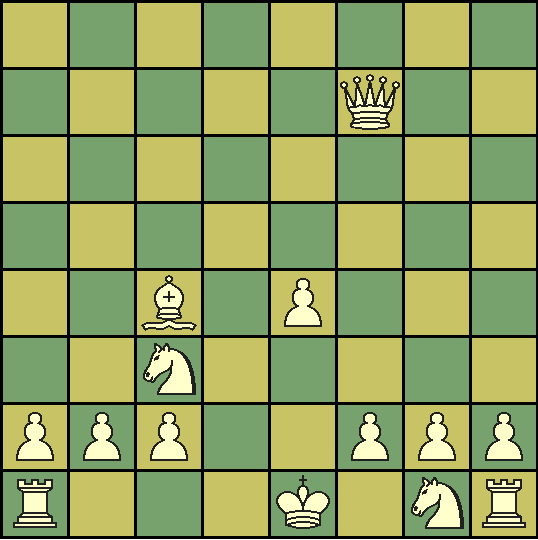
\includegraphics[width=0.7\textwidth]{images/OneView.png}
\caption{White's view}
\label{fig:figure2}
\end{minipage}
\vspace{-0.2in}
\end{figure}


%\begin{figure}
%\begin{verbatim}
%1. d4 {(:)}
%   a5 {(:)}
%2. Bg5 {(:)}
%   b6 {(:)}
%3. Nc3 {(:Bd8)}
%   c5 {(:)}
%4. d5 {(:Bd8;Tc5)}
%   Na6 {(:)}
%5. d6 {(:)}
%   f6 {(:Td6)}
%6. e4 {(:)}
%   fxg5 {(Xg5:Td6;Tg5)}
%7. Bc4 {(:)}
%   exd6 {(Xd6:Td6)}
%8. Qd5 {(:)}
%   Qc7 {(:)}
%9. Qf7+ {(:)} 
%   d8 {:g6,f7,e7}
%10. Qxf8++ {(1-0:)}
%\end{verbatim}
%\label{listing}
%\caption{Listing of a kriegspiel game resulting in checkmate by white after 10 moves.}
%\end{figure}

\Section{Information Set Generation}
%\subsection{Information Set Generation}
The concept of information sets is perhaps best explained through an example. 
Figure~\ref{listing} and show a full listing and the associated pictorial progression of an actual
kriegspiel game~\cite{li94chess}.  We have adapted the notation used by Wolfe for Berkeley Kriegspiel.  Odd (resp. even) moves are for white (resp. black).  The actual move is shown
first followed by a list of referee announcements.  Captures announcements are prefixed with an X and give the location
of the captured piece.  Similarly, pawn tries announcements are prefixed with T.  Attempted moves that were ultimately
declared illegal are shown in a list following the `:'.  For example at move 9, (Figure~\ref{fig:9W}--\ref{fig:9B}),
black attempts to block a potential threat along the diagonal by moving a pawn to f6, then attempts to escape or capture
a threat at f7.  When both of these attempts fail, black can infer that his king is being threatened by a protected
bishop or queen at f7.  The attempt to move to e7 is black's way of finding out whether the threatening piece is a queen
or bishop.  When this move fails, black knows it is white's queen and ultimately retreats to d8.  Note that the failed
moves by white on turns 3 and 4 are a result of being blocked by the pawn at e2.


The listing in Figure~\ref{listing} corresponds to the referee's view of the game and would be useful for
post-game analysis or commentary.  During the game, players would not have access to the full information.  The
transcript from white's perspective is shown in Figure~\ref{filteredlisting}.  Note that black's actual moves have been
replaced with ``??'' and lists of black's illegal moves have been replaced with the {\em number} of illegal attempted
moves.  For example, on move 9, black attempted three illegal moves.
\begin{figure}
\begin{minipage}[b]{0.35\linewidth}
\centering
\small
\begin{verbatim}
1. d4 {(:)}
   ?? {(:0)}
2. Bg5 {(:)}
   ?? {(:0)}
3. Nc3 {(:Bd8)}
   ??  {(:0)}
4. d5 {(:Bd8;Tc5)}
   ??  {(:0)}
5. d6 {(:)}
   ?? {(:0,Td6)}
\end{verbatim}
\end{minipage}
\begin{minipage}[b]{0.25\linewidth}
\small
\centering
\begin{verbatim}
6. e4 {(:)}
   fxg5 {(Xg5:Td6;Tg5)}
7. Bc4 {(:)}
   ?? {(Xd6:Td6)}
8. Qd5 {(:)}
   ?? {(:0)}
9. Qf7+ {(:)} 
   ?? {:0}
10. Qxf8++ {(1-0:)}
\end{verbatim}
\end{minipage}
\vspace{-0.1in}
\caption{Listing of a kriegspiel game resulting in checkmate by white after 10 moves.}
\label{filteredlisting}
\vspace{-0.2in}
\end{figure}

The listing of a sequence of moves from the perspective of one player lists all of that player's moves exactly and
includes the declarations from the referee.  We refer to such a list as a player's observations.  Given a list of
observations for a sequence of moves, an information set is the set of all possible {\em sequences of moves for both
players}, that are consistent with those observations.  In other words, any sequence of moves that would have generated
the same sequence of observations for black is in black's information set.  Figure~\ref{abbrevoutput} shows the
information set for black after both player's have made five moves.  From this list of possibilities, black can infer
that white must have a bishop at g5 and a pawn at d6.  There are 25 possible sequences of moves that are consistent with
black's observations up to that point. 

%Table~\ref{bothtimes} shows the size of the information sets for each player for
%each move in the game and the amount of time to find the full set on a single processor.  Appendix B shows the full
%output of the program for the same point in the game (five moves for each player) and illustrates all of the possible
%positions in the belief state.

\begin{figure}
\begin{mytinylisting}
1. Pa2:a4 Pa7:a5 2. Pd2:d4 Pb7:b6 3. Bc1:g5 Pc7:c5 \\
4. Pd4:d5 Nb8:a6 5. Pd5:d6 Pf7:f6 \\
\\
1. Pd2:d3 Pa7:a5 2. Bc1:g5 Pb7:b6 3. Pd3:d4 Pc7:c5 \\
4. Pd4:d5 Nb8:a6 5. Pd5:d6 Pf7:f6 \\
\\
1. Pd2:d4 Pa7:a5 2. Pa2:a4 Pb7:b6 3. Bc1:g5 Pc7:c5 \\
4. Pd4:d5 Nb8:a6 5. Pd5:d6 Pf7:f6 \\

%1. Pd2:d4 Pa7:a5 2. Bc1:f4 Pb7:b6 3. Bf4:g5 Pc7:c5 4. Pd4:d5 Nb8:a6 5. Pd5:d6 Pf7:f6 \\
%1. Pd2:d4 Pa7:a5 2. Bc1:g5 Pb7:b6 3. Pa2:a3 Pc7:c5 4. Pd4:d5 Nb8:a6 5. Pd5:d6 Pf7:f6 \\
%1. Pd2:d4 Pa7:a5 2. Bc1:g5 Pb7:b6 3. Pa2:a4 Pc7:c5 4. Pd4:d5 Nb8:a6 5. Pd5:d6 Pf7:f6 \\
%1. Pd2:d4 Pa7:a5 2. Bc1:g5 Pb7:b6 3. Pb2:b3 Pc7:c5 4. Pd4:d5 Nb8:a6 5. Pd5:d6 Pf7:f6 \\
%1. Pd2:d4 Pa7:a5 2. Bc1:g5 Pb7:b6 3. Pc2:c3 Pc7:c5 4. Pd4:d5 Nb8:a6 5. Pd5:d6 Pf7:f6 \\
%1. Pd2:d4 Pa7:a5 2. Bc1:g5 Pb7:b6 3. Pe2:e3 Pc7:c5 4. Pd4:d5 Nb8:a6 5. Pd5:d6 Pf7:f6 \\
%1. Pd2:d4 Pa7:a5 2. Bc1:g5 Pb7:b6 3. Pe2:e4 Pc7:c5 4. Pd4:d5 Nb8:a6 5. Pd5:d6 Pf7:f6 \\
%1. Pd2:d4 Pa7:a5 2. Bc1:g5 Pb7:b6 3. Pf2:f3 Pc7:c5 4. Pd4:d5 Nb8:a6 5. Pd5:d6 Pf7:f6 \\
%1. Pd2:d4 Pa7:a5 2. Bc1:g5 Pb7:b6 3. Pf2:f4 Pc7:c5 4. Pd4:d5 Nb8:a6 5. Pd5:d6 Pf7:f6 \\
%1. Pd2:d4 Pa7:a5 2. Bc1:g5 Pb7:b6 3. Pg2:g3 Pc7:c5 4. Pd4:d5 Nb8:a6 5. Pd5:d6 Pf7:f6 \\
%1. Pd2:d4 Pa7:a5 2. Bc1:g5 Pb7:b6 3. Pg2:g4 Pc7:c5 4. Pd4:d5 Nb8:a6 5. Pd5:d6 Pf7:f6 \\
%1. Pd2:d4 Pa7:a5 2. Bc1:g5 Pb7:b6 3. Ph2:h3 Pc7:c5 4. Pd4:d5 Nb8:a6 5. Pd5:d6 Pf7:f6 \\
%1. Pd2:d4 Pa7:a5 2. Bc1:g5 Pb7:b6 3. Ph2:h4 Pc7:c5 4. Pd4:d5 Nb8:a6 5. Pd5:d6 Pf7:f6 \\
%1. Pd2:d4 Pa7:a5 2. Bc1:g5 Pb7:b6 3. Nb1:a3 Pc7:c5 4. Pd4:d5 Nb8:a6 5. Pd5:d6 Pf7:f6 \\
%1. Pd2:d4 Pa7:a5 2. Bc1:g5 Pb7:b6 3. Nb1:c3 Pc7:c5 4. Pd4:d5 Nb8:a6 5. Pd5:d6 Pf7:f6 \\
%1. Pd2:d4 Pa7:a5 2. Bc1:g5 Pb7:b6 3. Nb1:d2 Pc7:c5 4. Pd4:d5 Nb8:a6 5. Pd5:d6 Pf7:f6 \\
%1. Pd2:d4 Pa7:a5 2. Bc1:g5 Pb7:b6 3. Qd1:d2 Pc7:c5 4. Pd4:d5 Nb8:a6 5. Pd5:d6 Pf7:f6 \\
%1. Pd2:d4 Pa7:a5 2. Bc1:g5 Pb7:b6 3. Qd1:d3 Pc7:c5 4. Pd4:d5 Nb8:a6 5. Pd5:d6 Pf7:f6 \\
%1. Pd2:d4 Pa7:a5 2. Bc1:g5 Pb7:b6 3. Qd1:c1 Pc7:c5 4. Pd4:d5 Nb8:a6 5. Pd5:d6 Pf7:f6 \\
%1. Pd2:d4 Pa7:a5 2. Bc1:g5 Pb7:b6 3. Ke1:d2 Pc7:c5 4. Pd4:d5 Nb8:a6 5. Pd5:d6 Pf7:f6 \\
%1. Pd2:d4 Pa7:a5 2. Bc1:g5 Pb7:b6 3. Ng1:f3 Pc7:c5 4. Pd4:d5 Nb8:a6 5. Pd5:d6 Pf7:f6 \\
%1. Pd2:d4 Pa7:a5 2. Bc1:g5 Pb7:b6 3. Ng1:h3 Pc7:c5 4. Pd4:d5 Nb8:a6 5. Pd5:d6 Pf7:f6 \\
\end{mytinylisting}
\vspace{-0.2in}
\caption{Abbreviated output from example game.  Generating information sets for black after five turns by each player.
From this, black can infer that there is definitely a white bishop at g5 and a white pawn at d6.}
\label{abbrevoutput}
\vspace{-0.3in}
\end{figure}

%\begin{table}
%\centering
%\begin{tabular}{rrrrr}
% & \multicolumn{2}{c}{\bf White} & \multicolumn{2}{c}{\bf Black} \\
%{\bf Ply} & {\bf Size} & {\bf Time} & {\bf Size} & {\bf Time} \\
%1 & 18 & 0.000 & 20 & .000 \\
%2 & 18 & 0.000 & 19 & .000 \\
%3 & 18 & 0.000 & 404 & .008\\
%4 & 279 & 0.008 & 401 & .024\\
%5 & 242 & 0.028 & 1472 & .044\\
%6 & 216 & 0.052 & 155 & .096\\
%7 & 176 & 0.064 & 293 & .116\\
%8 & 3406 & 0.092 & 158 & .128\\
%9 & 2191 & 0.288 & 118 & .148\\
%10 & 1423 & 0.508 & 25 & .152\\
%11 & 1363 & 0.596 & 798 & .164\\
%12 & 1416 & 0.744 & 518 & .192\\
%13 & 1416 & 0.836 & 13564 & .304\\
%14 & 3440 & 0.97 & 12394 & .776\\
%15 & 3428 & 1.25 & 343652 & 3.75\\
%16 & 50521 & 1.82 & 320704 & 17.3\\
%17 & 43192 & 5.91 & 490162 & 99.9\\
%18 & 26128 & 7.94 & 3792 & 119\\
%19 & 19061 & 9.92 & 14836 & 121\\
%\end{tabular}
%\caption{Solution counts and running times for a sample kriegspiel game}
%\label{bothtimes}
%\end{table}

%Table~\ref{sampletimes}
%\begin{table}
%\begin{tabular}{ccc}
%1 & 20 & .000\\
%2 & 19 & .000\\
%3 & 404 & .008\\
%4 & 401 & .024\\
%5 & 1472 & .044\\
%6 & 155 & .096\\
%7 & 293 & .116\\
%8 & 158 & .128\\
%9 & 118 & .148\\
%10 & 25 & .152\\
%11 & 798 & .164\\
%12 & 518 & .192\\
%13 & 13564 & .304\\
%14 & 12394 & .776\\
%15 & 343652 & 3.75\\
%16 & 320704 & 17.3\\
%17 & 490162 & 99.9\\
%18 & 3792 & 119\\
%19 & 14836 & 121 \\
%\end{tabular}
%\caption{Solution counts and running times for a sample kriegspiel game}
%\label{blacktimes}
%\end{table}

   
\textbf{The Information Set Generation Algorithm}
(ISG) can be formulated as a combinatorial search problem.  The input to the algorithm is a list
of observations for one player in a kriegspiel game.    

The nodes in the search tree at depth $n$ correspond possible to possible sequences of $n$ plies from the start state.
There is a search space variable for each ply in the game, and the values that a variable can take on are all possible
legal moves.  Information set generation, then, is an all-solutions search through the space.  Whenever a node in the search tree is
found to be inconsistent with the actual observation given in the input, the
subtree rooted at that node is pruned (i.e., search is discontinued along that
path).  There are types of observations that must match in order for the state
to be found: check status, pawn tries, and illegal moves available/attempted.

Figure~\ref{codelisting} shows the function at the heart of our information set generation algorithm.  The actual
observations can be viewed as global, read-only variables.  All solutions (i.e., all nodes in the information set) will
be located at the same depth in the tree: the depth that is equal to the number of plies in the observation list.
Referee announcements regarding pawn tries or a player being in check are made prior to a move.  The algorithm checks
for the consistency of these observations at line $7$.  If the search reaches the appropriate depth and passes these
tests, then a solution has been found and is added to the information set (line $3$).  

%Otherwise, we consider the possible moves that can be made from that state.  If the player whose turn it is to move at
%the current level of the search tree is the same player from whose perspective we have received observations, then the
%next step is to make sure that every legal move that was attempted at the player at that ply is also at least
%attemptable at the game position that corresponds to the game tree node (lines $15--22$).  We know exactly the legal
%move that was ultimately made at this depth (because we are assuming perfect recall), and we check to make sure that
%this move is indeed legal (pruning otherwise).  If so, we apply that move and recurse (lines $24--32$).  This
%corresponds to a ``forced move'' in the general search paradigm.
%
%On the other hand, if the player whose turn it is to move at the current depth of the search tree is the opponent, then
%must consider all possible legal moves to branch on.  We first check to make sure that the number of legal moves from
%this position is at least as large as the number of illegal moves that the opponent attempted (i.e., the number of times
%the referee said ``No'' before finally accepting the opponent's move).  This is shown in lines $39--42$.  At this point
%we generate a child for each move that would be accepted by the referee and recurse (lines $44--52$).
%
%One of our goals was to assess the varying utilities of the different pruning criteria.  We tried some different
%orderings of the tests and were somewhat surprised (and disappointed) to see that there was actually a fairly minimal
%impact on performance.  This could be due to the fact that because of the tedious nature of encoding problem instances
%from actual games, we were not able to run experiments of a wide variety of types of positions (i.e., different styles
%of play).

%\begin{figure}
%%\begin{listing}
%\begin{lstlisting}
%void generateInformationSet(uint16_t* trueState, uint16_t* possState, bool whiteMove, 
%	uint16_t* possHistory, uint16_t** levels, int depth)
%{
%  if (!samePawnTries(trueState, possState, whiteMove)) return;  
%  if (!sameCheckStatus(trueState, possState, whiteMove)) return; 
%  if (depth == maxdepth) { // Then we have found a solution
%	nSolutions++; return; // Report solution
%  }
%  uint16_t newPossState[16]; 
%  int nMoves = 0;
%  generateAttemptableMoves(possState, whiteMove, levels[depth], nMoves,false);
%  checkForCheck(possState, whiteMove, levels[depth], nMoves); // prunes if not equal
%  assert (nMoves < NMOVES); // 
%
%  if (whitePerspective == whiteMove) { // move from perspective plyaer 
%    SetMove& failures = failedMoves[depth];
%    for (SetMove::const_iterator itr = failures.begin(); itr != failures.end(); ++itr) {
%      uint16_t move = *itr ;
%      if (!foundMatchingMove(move,levels[depth],nMoves)) {
%        return; // Prune: one of my own failed moves is not attemptable in this state
%      }
%    }
%    // We know exactly what the actual move was; make it
%    uint16_t& actualMove = moveHistory[depth];
%    if (!foundMatchingMove(actualMove,levels[depth],nMoves)) {
%      return; // Prune (because the move that we know we made at this depth is not legal)
%    }
%    // Otherwise, recurse 
%    applyMove(possState,newPossState,actualMove);
%    possHistory[depth] = actualMove;
%    generateInformationSet(newTrueState, newPossState, !whiteMove, 
%      possHistory, levels, depth+1);
%  } else { 
%    // We are at a level in the search tree where 
%    // we are considering the possible moves for the opponent.
%    // We know the number of attempted illegal moves, but not which ones
%
%    // Must be enough attemptable moves in the state to match the number of failed attempts
%    unsigned nIllegalMoves = countIllegalMoves(levels[depth], nMoves);
%    if (nIllegalMoves < failedMoves[depth].size()) {
%	return; // Prune if not enough attemptable moves
%    }
%    // Now we want to try each possible move that is legally executable (not just attemptable) 
%    for (int i = 0; i < nMoves; i++) {
%      uint16_t& move = levels[depth][i];
%      if (isLegal(move)) { // Obviously, we can only execute the moves that are actually legal from this state
%        applyMove(possState,newPossState,move);
%        possHistory[depth] = move;
%        generateInformationSet(newTrueState, newPossState, !whiteMove, 
%          possHistory, levels, depth+1);
%      }
%    }
%  }
%}
%\end{lstlisting}
%\caption{The heart of the information set generation algorithm.}
%\label{codelisting}
%\end{figure}

\begin{figure}[htpb]
\small
%\begin{algorithm}
\begin{boxedminipage}{\columnwidth}
\begin{algorithmic}[1]
\Function{DFS-Infoset}{$a_{1:t}$, $o_{1:T}^{(k)}$, $I$, $s$, $t$}
  \If {$t > T$}
    \State {$I \leftarrow I \cup a_{1:t}$} %\Comment{$a_{1:t}$ leads to $o_{1:T}$ for $P_k$; add it to the information set.}
  \Else {
    \For{\textbf{each} legal action $a$ at $s$}
      \State {$s'$ = {\sc GetNextState}($s$,$a$)}\label{line:update}
      \If {$s'.o_{t+1}^{(k)}=o_{t+1}^{(k)}$}
        \State {{\sc DFS-Infoset}($a_{1:t}a$, $o_{1:T}^{(k)}$, $I$, $s'$, $t+1$)} 
          %\Comment{ Recall that $N(a_{1:t}a) = T(T(a_{1:t}),a)$}
      \EndIf
    \EndFor
  }\EndIf
\EndFunction
\label{codelisting}
\end{algorithmic}
\end{boxedminipage}
\caption{Algorithm}
\end{figure}

\Section{Parallel Implementation using Charm++ and ParSSSE}\label{ParSSSE}
We built our search engine on top of the {\sc Charm++} run-time
system for parallel processing~\cite{kale93charm,kale09charm}.  {\sc Charm++}
is an extension to the C++ programming language that provides
machine-independent infrastructure for parallel computation.  The language and
its accompanying runtime system have been ported to many shared-memory and
distributed-memory platforms.

In contrast to other popular parallel programming frameworks such as {\sc MPI}
and {\sc OpenMP}, the {\sc Charm++} language is based on object-oriented
programming principles.  The programmer is responsible to decompose its problem
into a collection of objects that represent elements of work to be done.
Typically the number of work objects far exceeds the number of processing
elements (cores) available.  These objects are defined so as to be able to be
migrated between processors {\em during execution}, in order to improve the
overall load balancing.  

Work objects, known as {\em chares}, communicate with each other via
asynchronous message-passing.  Objects can invoke {\em entry methods} on other
objects, which are executed according to a schedule set by the {\sc Charm++}
runtime system.  The runtime is responsible to interleave computation and
communication tasks in order to maximize efficiency.  To facilitate this, each
processor maintains an {\em incoming queue} of messages targeted to chares that
it currently holds.  A corresponding {\em outgoing queue} collects messages
generated by objects on the processor that need to be sent to objects assigned
to other processors.

Some work tasks may inherently require more computation than others, but the
amount of computation associated with each piece of work is not always known
before execution.  In tree search, for example, a piece of work may be defined
as the computation of a minimax value on a node in the tree using alpha-beta
pruning.  A natural decomposition is to assign different nodes to different
processors for evaluation.  Because some nodes will be pruned at shallower
levels of the tree than others, the amount of work performed at each subtree can
vary considerably.  In a traditional parallel framework, this would result in
many processors idling while a small number of processors execute the larger
workloads. By allowing the {\sc Charm++} runtime system to schedule a large
number of small pieces of work, better adaptive load balancing is achieved. 

%\subsection{The {\sc Charm++} Parallel State Space Search Engine}
Sun \etal have developed the Parallel State Space Search Engine ({\sc ParSSSE})
within the {\sc Charm++} framework, which exposes an API that is useful for a
variety of graph-based and tree-based search problems~\cite{sun11adaptive}. In
{\sc ParSSE} the fundamental unit of work is the processing of a node.
Generally, this means identifying whether the node corresponds to a solution
and/or generating descendant nodes and spawning work tasks related to them. A
task is {\em terminal} if it spawns no children. 

A {\em grainsize control} parameter specifies a bound on the size of a piece of
work that can be passed along to the runtime system for scheduling.  Once a
task has been subdivided into an appropriate number of subtasks, those tasks
run to completion on a single processor without preemption and without generating
any additional parallel tasks.  If the grainsize is too large, then the number
of pieces of work to be done may be lower than the number of processors
available, forcing some processors to idle.  If the grainsize is too small,
then the runtime system is flooded with a large number of trivial tasks, and
the system gets bogged down by the overhead of creating and scheduling tasks
instead of actually doing them.  {\sc ParSSE} supports an adaptive grainsize
management, so that the threshold for sequential processing can be changed
during the execution of the program, depending on the properties of the problem
and/or the realtime performance analysis of the runtime system.

{\sc ParSSE} currently supports two different load balancing strategies.  The
first is the randomized strategy.  In this approach, each newly created object
is assigned to a random processor.  Generally, if a large enough number of 
chares is created, the system will achieve an approximately uniform
distribution of work across processors.  The approach is also appealing because
of its simplicity. However, randomization can sometimes lead to inefficiencies
from parallel overhead.  For a program running on $p$ processors, the
probability that a piece of work is assigned to a processor other than the
one that created it is $1-1/p$.  As the number of processors gets large, this
probability approaches 1, which means that the parallel overhead related to the
creation and scheduling of a new task is incurred for almost every piece of new
work.
 
A second load balancing strategy is known as {\em work stealing}.  In this
approach, all new tasks are inserted in the message queue of the processor that
spawns them.  Whenever a processor is idle it becomes a {\em thief}.  A thief
randomly selects another processor as its {\em victim} and sends a message to
that processor requesting work.  When the victim receives the message, it
removes the work with the highest priority from its own queue and sends it to
the thief.  If it has no work available, it sends a negative acknowledgment
message to the thief, which causes the thief to look for another victim.

The advantage of the work stealing strategy is that the message-passing
overhead is only incurred if at least one processor is idling.  Furthermore,
because victims respond by sending the highest priority work, the most
important tasks are more likely to get done sooner.  

In addition to these strategies, a user may define its own load balancing
strategies by overriding {\sc Charm++} task dispersal functions.


\Section{Performance Results}\label{Results}
In order to understand the effect of various parameters such as grain size and load balancing, we first evaluated the scalability of our implementation using a randomly selected problem instance. Next, we show that our implementation performs equally well for instances from actual games.
\subsection{Analysis using Random Instance}
The performance results reported in
this section were obtained by running our program on Blueprint with up to 1024 processors. TODO: Blueprint H/w or citation

Table~\ref{speedups} shows the performance results for our algorithm on a randomly selected problem instance in which
the size of the information set was about 4.5 million.  This instance is not necessarily representative of all games or
states of the game, but it was not cherry-picked in any way. The table shows that the problem is indeed highly
parallizable.  The speedups are nearly linear for up  to 32 processors, and even on 1024 processors, we get a good
speedup.  In this particular instance, the sequential algorithm takes almost 25 minutes to run.  But when parallelized
on 1024 processors---perfectly reasonable resource usage on modern hardware---the search takes less than three seconds.
This is a speedup of 576 times!  It might not be reasonable to use the algorithm at all if it takes 25 or more to run
for some turns.  But if the cost is only a few seconds, it becomes entirely feasible.

\begin{table}
\centering
\begin{tabular}{rrr}
{\bf Procs}	&	{\bf Time (s)} 	&	{\bf Speedup}\\
1	&	1524	&	1\\
2	&	812	&	1.88\\
4	&	407	&	3.74\\
8	&	208	&	7.32\\
16	&	102	&	14.8\\
32	&	53.2	&	28.7\\
64	&	28.0	&	54.5\\
128	&	14.9	&	102\\
256	&	7.70	&	197\\
512	&	4.59	&	331\\
1024	&	2.64	&	576\\
\end{tabular}
\vspace{-0.1in}
\caption{Speedups for a randomly selected problem instance on 1--1024 processors.  The input observations were from the
10th ply of the game tree and the size of the information set in this instance is 4,495,121.}
\label{speedups}
\vspace{-0.3in}
\end{table}

\subsubsection{Effect of Load Balancing}
\begin{figure}[h]
\centering
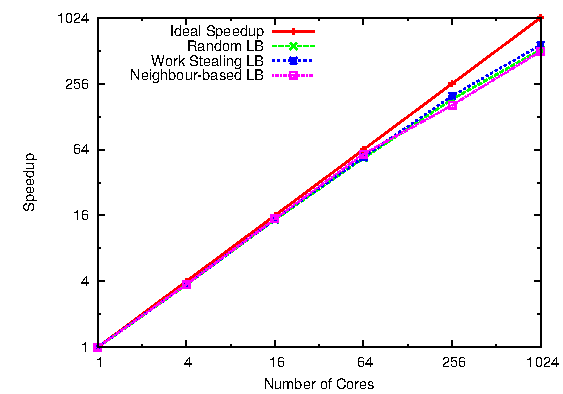
\includegraphics[width=0.7\columnwidth]{plots/3schemes.pdf}
\vspace{-0.1in}
\caption{Effect of load balancing strategy}
\label{3schemes}
\vspace{-0.2in}
\end{figure}

In our next round of experiments, we set out to compare a few different load-balancing strategies for the problem.  We
used the random, work stealing, and neighborhood balancing strategies that are available in the general purpose search
engine.  These results are shown in Figure~\ref{3schemes}.  Our results show that there was actually very little
variation in performance across the different strategies.  We did notice that across all of our experiments, the work
stealing approach appeared to be consistently---if only marginally---better than the others.  Our hypothesis here is
that perhaps the nodes are rarely starved for work.  In other words, perhaps the very nature of the problem means that
the load is naturally well-balanced and that the load-balancer rarely needs to do a significant amount of
redistribution.  This is probably also related to the fact that we are doing an all-solutions search. 

 
\subsubsection{Effect of Problem Size}
\begin{figure}[h]
\centering
\begin{minipage}{0.5\linewidth}
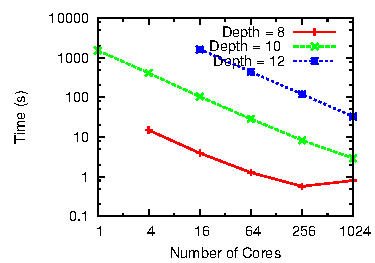
\includegraphics[width=\columnwidth]{plots/3depths.pdf}
\end{minipage}
\centering
\begin{minipage}{0.5\linewidth}
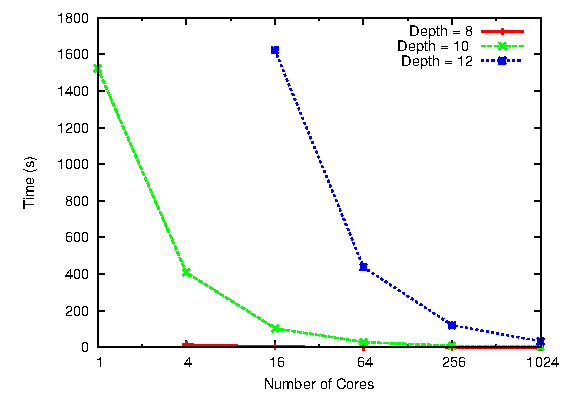
\includegraphics[width=\columnwidth]{plots/3depthsnolog.pdf}
\end{minipage}
\vspace{-0.1in}
\caption{(Top) Log-log plot of running time for three different sizes of problem as the number of cores used increases.
(Bottom) Same data with a linear y-axis for the running time (to help see the Iso-efficiency.)}
\vspace{-0.2in}
\label{3depths}
\end{figure}

We next study the variation in the efficiency of the parallelization of the
algorithm with {\em size} of the problem?  To test this, we varied the number of plies in the test instance from
8 to 12. We used the work stealing load balancing strategy.  The results are shown in Figure~\ref{3depths}.   In the easiest case (depth 8), there isn't
enough additional parallel work to justify the jump from 256 to 1024 processors, and performance actually degrades.
Other than that, however, we see consistent speedups as we increase the number of processors.  The plot on the right helps to
illustrate the good isoefficiency of the problem.  As the size of the problem increases, the amount of parallelizable
work available also increases, and therefore the steepness of the speed curve is higher for larger problem sizes, as the
number of processors increases.
 
\subsubsection{Effect of Grain Size}

\begin{figure*}[!ht]
\centering
\subfigure[Depth 8]{
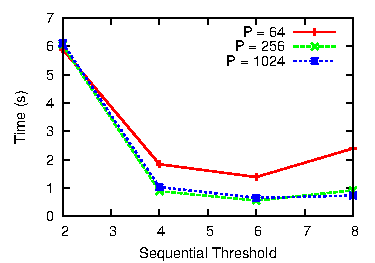
\includegraphics[width=2in]{plots/dep8.pdf}
\label{dep8}
} 
\subfigure[Depth 10]{
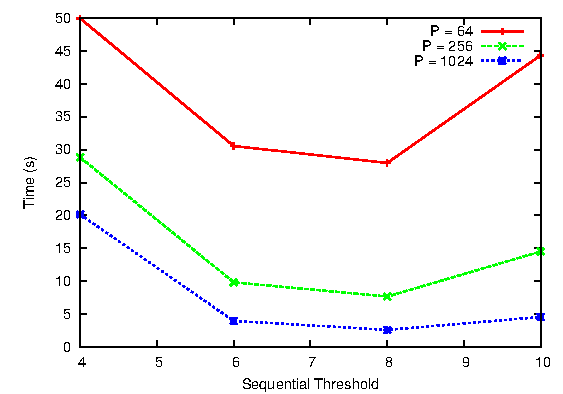
\includegraphics[width=2in]{plots/dep10.pdf}
\label{dep10}
} 
\subfigure[Depth 12]{
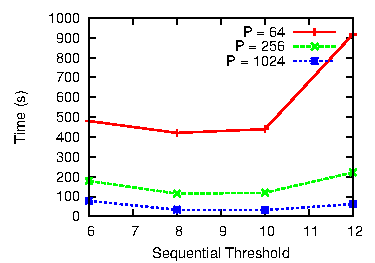
\includegraphics[width=2in]{plots/dep12.pdf}
\label{dep12}
} 
\vspace{-0.1in}
\caption{Grain Size Control for different problem sizes}
%\vspace{-0.1in}
\label{fig:dep}
\vspace{-0.1in}
\end{figure*}

Next, we evaluate the effect of grainsize on the problem execution time.  The results are shown in
Tables~\ref{dep8}--~\ref{dep12}.  It is clear that there is a ``sweet spot'' for each problem size.  (At least it is
clear for this particular instance.  It is possible that there would be different behavior on different problem
instances.)  When the grainsize is too small, the overall computation is hampered by excessive parallel overhead
(communication, queueing of nodes to expand, load balancing operations).  On the other hand, when the grain size is too
large, it becomes too difficult to ensure that all processors are busy and processors are not idling with no work to do
while a small number of processors are busy doing large-sized chunks of work.  

In our experiments, the optimal grainsize is clearly related to the size of the problem, the depth of the search tree.
The optimal sequential threshold seems to be $2--4$ less than the problem depth.  Since the depth of all solutions is
the same for each problem instance, this means that the number of levels that should be searched sequentially is fairly
consistent across problem sizes.  We noted that the number of solutions found---in other words, the size of the
information sets---is typically fairly large with respect to the total number of nodes expanded.  (We don't have hard
figures, but we estimate that it was often $30-40\%$).  This high density of solutions limits the variability that can
be present in the amount of work to be done at the nodes representing the last few levels of the tree.  This means that
the best grainsize is also likely to be fairly predictable.  


\subsection{Real Game Instance}
\begin{figure}[ht]
 \centering 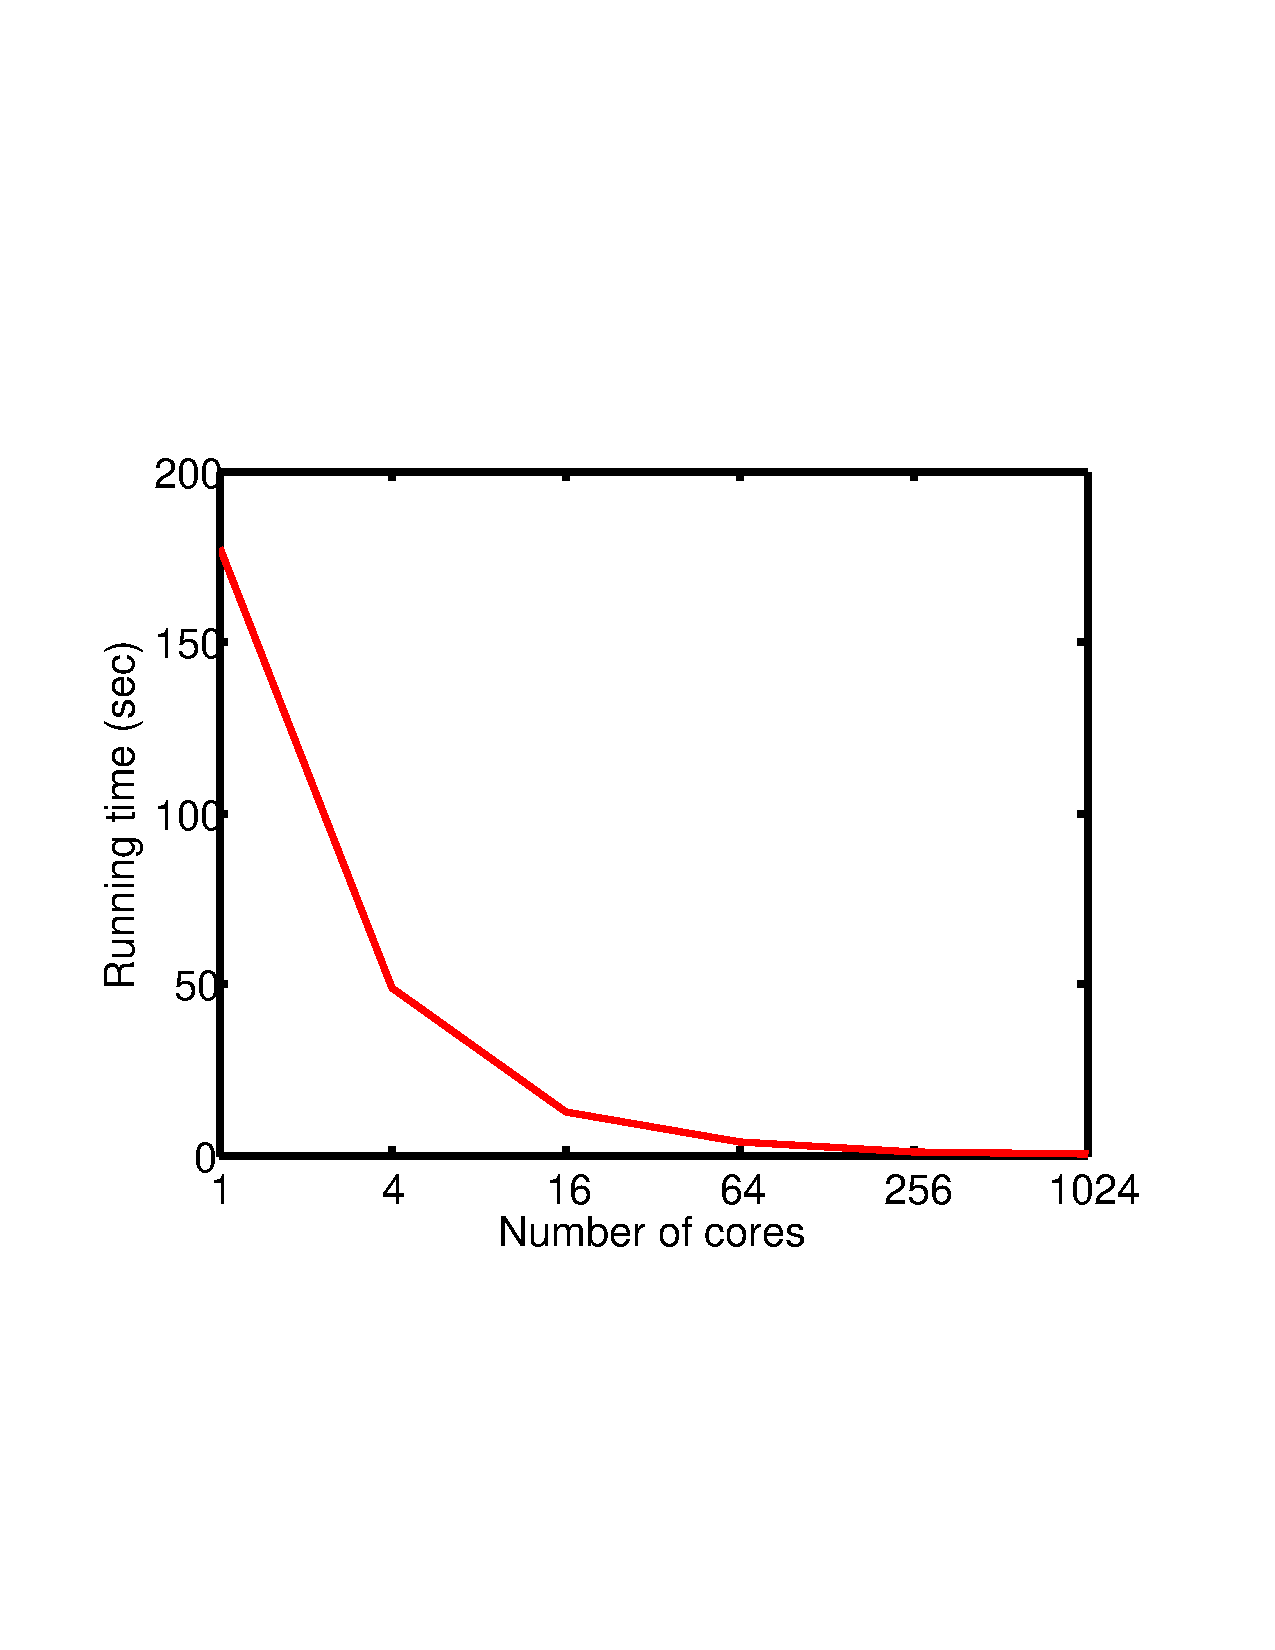
\includegraphics[viewport= 280 200 300 550, scale=0.35]{images/KriegspielProblem4.pdf} %
\caption{Kriegspiel position from Virgil-David 1969 with information set size 764,209.}
\label{prob4} 
\vspace{-0.2in}
\end{figure}

\begin{figure}[ht]
 \centering 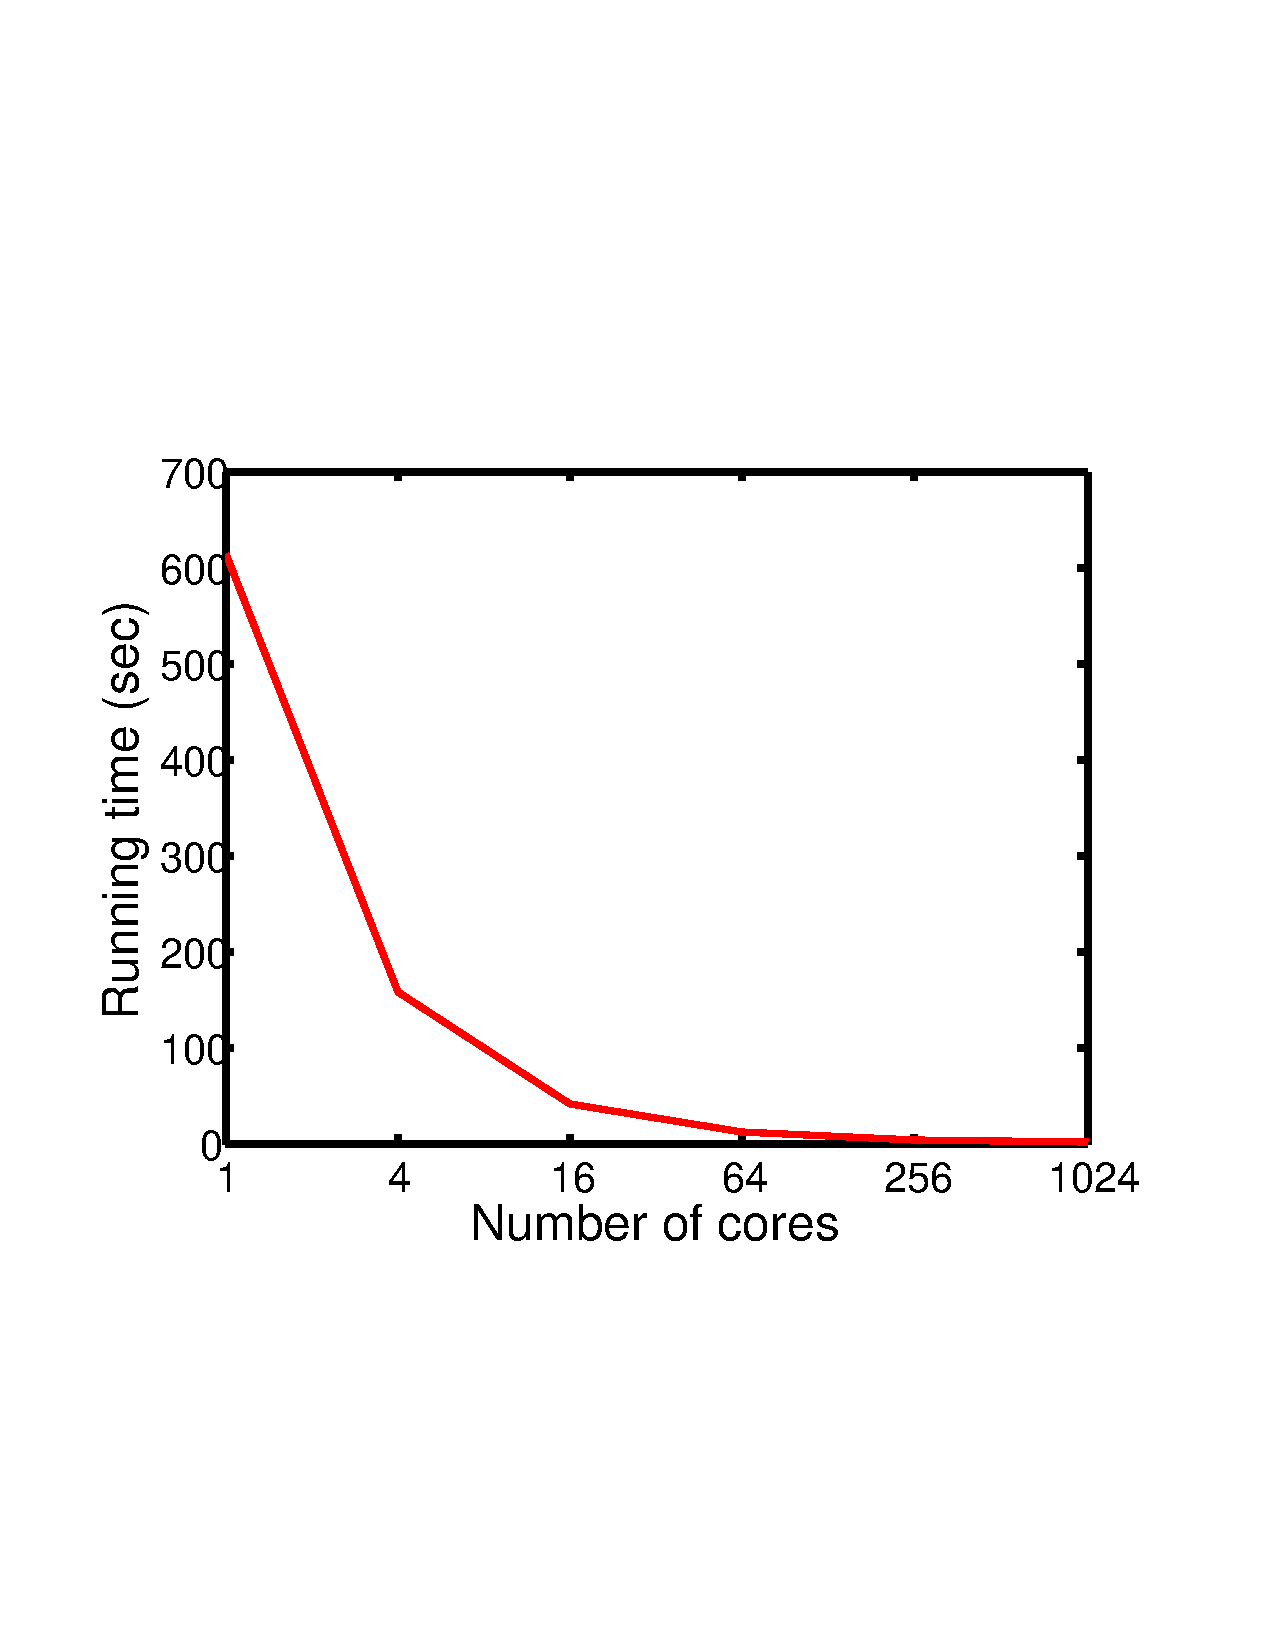
\includegraphics[viewport= 280 200 300 550, scale=0.35]{images/KriegspielProblem5.pdf} %
\caption{Kriegspiel position from Game 6 of Kbot-Darkboard at the 2006 Computer Chess championship.  Information set size is 5,099,257.}
\label{prob5} 
\vspace{-0.2in}
\end{figure}


We also evaluated our information set generation routine on 40 positions from actual kriespiel games, including human vs. human and computer vs. computer.  Many of these were trivial to solve in a few seconds or less on a desktop computer.  The running times and speedups for two of the more challenging instances are shown in Tables~\ref{prob4}--\ref{tab:prob5speedups}.  These tables show the results for runs on one to $1024$ cores.  Each column corresponds to a different parameter.  In this case, the grainsize is the number of levels of the search tree that are searched in parallel.  Up to that threshold, each node that is generated spawns a new piece of work, which the {\sc Charm++} runtime schedules to execute on one of the processing elements according to its load balancing strategy.  Above the threshold the entire subtree is searched to completion on a single processor, with no additional parallel overhead. 

Note that the optimal grainsize varies for the different numbers of cores and the pattern is relatively consistent across problem instances.  The optimal grainsize increases as the number of cores increases.  This makes sense, because as this parameter grows, the number of distinct pieces of work increases.  When the number of pieces of work per processor is high, much of the overhead of parallelization is wasted.  But as the number of cores increases, the work can be efficiently broken up into smaller pieces and doled out to all the cores.  With more pieces of work, it becomes easier to balance the load.

\begin{table}[tphb]
\centering
\begin{tabular}{rrrrr}
PE/G & 2 & 4 & 6 & 8 \\
1 & {\bf 177$|$1} & 178$|$0.99 & 1844$|$0.96 & 493$|$0.36 \\
4 & 71$|$2.48 & 53$|$3.34 & {\bf 48$|$3.63} & 75$|$2.35 \\
16 & 34$|$5.19 & 19 $|$9.27& {\bf 12$|$13.8} & 16$|$10.7 \\
64 & 24 $|$7.25 & 7 $|$23.6& {\bf 3.7$|$47.39} & 4.1$|$43.1 \\
256 & 24 $|$ 7.1& 4.4 $|$40.1 & 1.2 $|$145& {\bf 1.0$|$172} \\
1024 & 26 $|$6.61 & 3.8 $|$46.5& 0.64 $|$276& {\bf 0.40$|$443}
\end{tabular}
\caption{Running times in seconds and speedups (after $|$), to find full information set of size 764,209 at position 10 of Virgil-David 1969. Optimal grainsize (G) for each number of cores (PE) is shown in bold}
\vspace{-0.2in}
\label{tab:prob4}
\end{table}

\begin{table}[tphb]
\centering
\begin{tabular}{rrrrr}
PE/G & 2 & 4 & 6 & 8 \\
1 & 617$|$1 & {\bf 612$|$1} & 650$|$0.95 & 3312$|$0.19 \\
4 & 213$|$2.89 & 170$|$3.63 & {\bf 158$|$3.89} & 367$|$1.68 \\
16 & 83$|$7.41 & 49$|$12.4 & {\bf 40$|$15.1} & 64$|$9.57 \\
64 & 54$|$11.3 & 19$|$32.3 & {\bf 11$|$52.9} & 14.9$|$41.4 \\
256 & 54$|$11.3 & 9.8$|$62.9 & 3.5$|$172 & {\bf 3.5$|$174} \\
1024 & 58$|$10.6 & 5.5$|$111 & 1.3$|$464 & {\bf 1.2$|$536} \\
\end{tabular}
\caption{Running times, in seconds and speedups (after $|$), to find full information set of size 5,099,257 at position 10 of Game 6 Kbot-Darkboard 2006. Optimal grainsize for each number of cores is shown in bold.}
\vspace{-0.2in}
\label{tab:prob5}
\end{table}

Note that both problems scale well even up to 1024 processors.  We achieve a speedup of $443$ in the game between humans and up to $536$ in the game between computers.  Figures~\ref{prob4} and~\ref{prob5} show the plots of the running times for the best grainsize for each core setting.  These plots show that the running time continues to decrease as the number of cores increases.

Our results compare favorably to previous work in parallel game tree search, shown in Table~\ref{bestspeedups}.  The previous best parallelization results were for parallelizing alpha-beta pruning.  Ferguson and Korf achieved a speedup of 12 on 32 cores in the game of Othello~\cite{ferguson88distributed}.  In the game of chess, Felton and Otto showed a speedup of 100 on 256 cores~\cite{felten88highly}.  This limited scalability is due to speculative loss.  Parts of the game tree that are searched during the parallel execution would have been pruned had the algorithm run sequentially.  This is a fundamental limitation in alpha-beta search. 

For partially observable games, information set generation represents a different variety of tree search that does not suffer from speculative loss.  All of the nodes that are visited in parallel would have also been visited in a sequential run.  The key challenge for parallelizing information set generation is load balancing: some parts of the tree will be pruned at a higher level than others, resulting in a wide variation in cost for each subtree.  The {\sc Charm++/ParSSSE} framework is perfectly suited to handle the load balancing issues that this problem naturally presents.

Note also that information set generation is just one subroutine needed to reason about partially observable games.  Once plausible game histories have been found, an agent may simulate some sequences of moves up to previous moves made by opponents and then recursively call the information set generation procedure from the perspective of the opponent.  This results in many parallel applications of information set generation. Furthermore, given a node in an information set, it is common for an agent to perform forward search on that node (e.g., using MCTS).  With these two additional levels of parallelism on top of the information set generation problem, it is conceivable that the problem of playing partially observable games could scale efficiently to millions of processors or more.
\begin{table}[tphb]
\centering
\begin{tabular}{lrrc}
{\bf Authors} & {\bf Game} & {\bf Year} & {\bf Best Speedup (cores)} \\
Ferguson \& Korf & Othello & 1988 & 12(32) \\
Felton \& Otto & Chess & 1988 & 100(256) \\
Richards \etal & Kriegspiel & 2012 & 178(256) \\
Richards \etal & Kriegspiel & 2012 & {\bf 536(1024)} \\
\end{tabular}
\caption{Best Speedups reported for game tree applications.}
\vspace{-0.2in}
\label{bestspeedups}
\end{table}

\Section{Related Work}
An overview of the theory of imperfect information games and other basic topics in game theory can be found
in~\cite{kuhn03lectures} and~\cite{kuhn97classics}.  A technical explanation of the concept of information sets can be
found in~\cite{gilpin07algorithms}.  Koller \etal, showed that a Nash
equilibrium can be found in time that is polynomial in the number of nodes in the game tree~\cite{koller94fast}.  In fact, they found
that it took about as much time to generate the full game tree as it did to actually solve it.  Unfortunately, this is
feasible only for small games.  In larger games where theoretically optimal strategies cannot be computed efficiently,
computer systems tend to utilize the concept of information sets or belief states in some form or another.  A common
strategy is to estimate the value of a move by averaging the estimated value of the associated descendant for each node
in the current information set (or a random sample from the set).  While this sort of ``averaging over clairvoyance''
{\em can} lead to very poor decisions, it is nevertheless a reasonable strategy in some games (e.g.,
Scrabble~\cite{sheppard02world}).

In this work, we have argued for an information set generation approach to kriegspiel, but other authors have approached
the problem differently.  Parker \etal, consider the problem of sampling from belief states in a variety of large game
trees, including kriegspiel~\cite{parker05game}.  They show that some performance gains can be achieved by only
approximate sampling from the belief state.  Instead of generating the full information set, or even sampling from it,
they sample from possible positions for the current state (i.e., sampling from the belief state) by matching only the
most recent observations.  The motivation for this approach seems to be that it would not be feasible to sample from
the full information set, because of the computational expense involved.  And indeed, our experiments bear this out-- it
can indeed be expensive to produce the full information set.  For the experiments shown in Table~\ref{speedups},
generating the full information set took over 25 minutes on a single processor.  However, by utilizing the Charm++
search engine on a parallel machine (1024 processors), we were able to generate the full set in just 2.9 seconds.  (Note
that this set had more than 4 million members.)  

%Li gives an overview of kriegspiel and discusses strategy from the perspective of human players~\cite{li94chess}.  He
%walks through the analysis of several actual games between two human players and discusses the inferences that each
%player can and should make at each position.  As in chess, human players are able to reason about the game at an
%abstract level; they tend to focus on a small number of critical possibilities and to emphasize the most important
%pieces and squares in each position.  Computer agents, lacking such sophistication, nevertheless have some advantages
%when it comes to brute force search strategies. Programs such Deep Blue have shown that a brute force approach to game
%tree search can be effective, even against humans with vastly superior abstract reasoning capabilities, provided that
%significant computational resources are available and wisely used~\cite{campbell02deep}.

%Russell and Wolfe have performed some analysis on kriegspiel positions for which it possible to prove that one player
%has a forced win (that is, regardless of the configuration of the opponent's unseen pieces, the player has a sequence of
%moves that is guaranteed to produce a checkmate)~\cite{russell05efficient, wolfe07exploiting}.  The authors assume
%knowledge of the player's belief state.  They claim that under certain "aggressive" styles of play, it is uncommon for
%information sets to exceed 10,000 nodes in size.  They throw out (i.e., do not analyze) any positions that exceed this
%threshold.  

%In our experiments, we have found positions in which the size of the information set is many tens of millions.  Our goal
%is to develop strategies that are amenable to use in this more general setting.   In other words, rather than being able
%to analyze positions only at the beginning or end of the game (when the size of the information set tends to be
%smaller), we want to be able to develop a strategy that can be used in the middle of the game as well.  game). 

The information set generation approach that we have presented is certainly also computationally expensive.  And
representing a full information set (e.g., as a list of sequences of moves that encode a path from the start state to
the current node) would be similarly expensive in terms of storage space.  However, we have shown that our algorithm is
also highly scalable.  Furthermore, contrary to the approach in~\cite{nance06reasoning}, our approach is readily
adaptable to sampling algorithms.  Given a sample size that matches available memory, any single sequence of moves is
readily extractable without the computational expense of a theorem prover or SAT solver.

%\Section{Conclusion Future Work}
%We have shown that information set generation for kriegspiel can be efficiently parallelized in a way that scales up to at least 1024 processors.

%A key line of future research is to use our ISG routine as part of a full Kriegspiel play.  The ISG method itself could be updated using constraint-satisfaction techniques outlined in ~\cite{richards12information}, which improve pruning performance in the search space by incorporating information from all observations in the list at each search step, instead of performing depth-first search.   The use of ISG-based opponent modeling to improve overall decision making is described in ~\cite{richards12reasoning}. 

%determined by how well that information improves a player's decision-making capabilities.  We noted earlier that a
%common use of information sets is to estimate the value of a move by averaging the estimated value of the associated
%descendant for each node in the current information set (or a random sample from the set).  This kind of strategy can be
%applied naively using a belief state sampling algorithm (i.e., an algorithm that samples from the distribution of
%possible worlds in the current state without respect to the overall history of moves).  However, it has been shown that
%significant improvement in play can be achieved by estimating the value of future moves from the perspective of the
%opponent, based on the knowledge that the opponent would have had at prior positions in the move
%history~\cite{richards07opponent}.  Such a strategy would require the use of an information set generation algorithm of the
%kind that we have described here.\footnote{This work is underway.}

%Ideally, we would run our algorithm on some deeper instances from real kriegspiel games.  We are not aware of a
%repository of such games.  Unfortunately, notation for kriegspiel is not standardized and there are several minor
%variations in rules (i.e., with respect to the nature of referee announcements) that are unlikely to significantly to
%impact the computability and scalability results but which nevertheless make it difficult to write an input reader that
%converts the transcript of a game into a sequence of moves readable by our algorithm.  An alternative would be to play
%some games ourselves.  Currently, the manual encoding of games is not difficult but is tedious.  Still, it would be nice
%to have some games that go on for 40 or 50 moves and have positions where the information sets are of moderate size (on
%the order of a few hundred thousand to a few million).

%The information set generation algorithm that we have implemented here is the most straightforward one and is alluded to
%in~\cite{parker05game} and~\cite{russell05efficient}.  It is analogous to the ``expand-at-the-tip'' strategy for the
%Hamiltonian Circuit problem.  An alternative information set generation algorithm is described
%in~\cite{richards09information} (but not implemented in parallel) and could potentially improve the search efficiency
%greatly by exploiting variable ordering.  This would be analogous to the disconnected edge-pairs\footnote{This is what we
%referred to as ``algorithm 2'' in class.} heuristic for the Hamiltonian Circuit problem.  Rather than search from the
%root node going forward, this algorithm would seek opportunities for pruning based on the propagation of logical
%consequences from each move both forward and backward in time.  This, incidentally, is more consistent with the way
%human players would analyze the game.  For example, if a player's proposed bishop move is rejected and the bishop is
%sufficiently removed from its own king, then the player may infer that one of his opponent's pieces is along that
%rejected path.  At least one of those spaces must have been the destination of a prior move by the opponent.  If a
%recent move by that bishop crossed the same path, then that would be hard evidence that those squares were empty at the
%time.  And therefore, the arrival of the opponent's piece must have been between the previous (successful) bishop move
%and the current (unsuccessful) bishop move.  To implement this algorithm, we envision the use of planning graph type
%data structures~\cite{blum97fast}.  Planning graphs have a sequence of alternating levels of state constraints and
%action constraints.  State constraints would be of the form $at(bishop,d4) \vee at(bishop,e6)$ or $!occupied(e4)$.
%Action constraints would be of the form $move(knight,a4,c5) \vee move(knight,e6)$.  At a minimum, each level would
%require a data structure with a bit for each possible action/state.  Propagating the constraints would require much of
%the same machinery used in STRIPS-like planning algorithms~\cite{chen05solving}, and one of the many knobs that would
%need to be tuned would be the depth of the propagation for each constraint.  (Should the consequences of a known action
%or non-action be propagated one move into the future and one move into the past?  More?  Less?)  Additionally, there
%would be a significant and interesting tradeoff in the effectiveness of pruning and the size of the data
%structures that would have to be encoded in each chare.  The best algorithm might be a hybrid strategy that does forward
%propagation from the root at the parallel level and constraint propagation at the sequential level.\footnote{This work
%is also in progress.}
%
%There are certainly several places where the efficiency of the details of each node expansion could be improved.  Many
%of these would reduce the overall running time but would not necessarily be interesting from the standpoint of
%evaluating the efficiency and isoefficiency of parallelization.  For example, in checking to see if a position leaves a
%player in check, we currently utilize existing helper functions that generate possible moves for the opponent.  It would
%be possible to write a more specialized function that focuses only on the position of the king in question and looks
%only at the squares along its rank, file, diagonals, and knight-edges for threats.  There are also some memory
%allocation issues that could be improved. 

\Section{Conclusion and Future Work}
We have shown that information set generation for kriegspiel can be efficiently parallelized.  The opportunities for
parallelism increase as the problem size increases.  Our algorithm has performed well on problems with information sets
with as many as 65 million nodes---much larger than any other treatment of the problem that we are aware of.  Because
the algorithm can be efficiently parallelized, it would be reasonable to explore using it in a full kriegspiel player.
It remains to be seen whether these scalability properties hold over a wide variety of playing styles and problem
instances.  We suspect that fruitful research remains with respect to alternative algorithms that implement variable
ordering heuristics.


%\Section{Appendix A}
%The purpose of this figure is simply to help visualize the concept of information sets in game trees.  The tree for
%kriegspiel is very difficult to visualize/depict (even an interesting part of the tree).  Figure~\ref{fulltree} shows
%the full game tree for a simple variant of poker known as Kuhn poker, which we hope will serve to at least make the
%concept clear, even if the poker game itself is not immediately relevant.  There are three cards: a king, a queen, and a
%jack.  The dealer deals one card to each of two players.  Each player antes one unit, and there is one simple round of
%betting, in which the size of the pot may be doubled.  Left branches denote check/fold; right branches denote bet/call.
%For this zero-sum game, terminal nodes are labeled with payoffs to player 1, whose decision points are shown in
%triangles.  Connections between nodes in the same information set are shown with dotted lines.  The top level shows
%three different information sets for the first player, one for each possible card that could be dealt to him.  There are
%two nodes in each set, because no matter what the deal is, there are two possibilities for the card that the other
%player holds.  The leftmost information set on the bottom level corresponds to player 1's observation that he was dealt
%a king and checked, and then the opponent wagered.  The second player has six information sets as well, but they are all
%at the same level of the tree.  Like the first player, the second player has a separate information set for each
%possible card that he could be dealt.  And the two nodes in each set are there because there are two possibilities for
%the opponent card.  The second player also gets to know whether the first player checked of bet, and that is why there
%are twice as many information sets.
%
%\begin{figure}
%\scalebox{.72}{
%\begin{tikzpicture}
%  [chance/.style={circle,draw=blue!50,fill=blue!20,thick,minimum size = 10mm},
%   terminal/.style={rectangle,draw=black!50,fill=black!20,thick, minimum size = 7mm},
%   maxer/.style={shape=regular polygon, regular polygon sides=3,draw=red!50,fill=red!30,thick,minimum size = 10mm,inner sep = 0pt},
%   miner/.style={shape=diamond,draw=green!50,fill=green!30,thick,minimum size = 10mm, inner sep = 0pt},
%   edge from parent/.style={red,thick,draw}, 
%   parent anchor=south,child anchor=north,
%   level 1/.style={sibling distance=4cm,level distance=1.4cm,
%       		growth parent anchor=south},
%   level 2/.style={sibling distance=2cm},
%   level 3/.style={sibling distance=1cm},
%   level 4/.style={sibling distance=1.0cm}]
%		\node  [chance] {}
%		    child {node (M1) [maxer] {\scalebox{.75}{K}}
%			child {node (M11) [miner] {\scalebox{.75}{Q-}}
%				child {node (M111) [terminal] {1}}
%				child {node (M112) [maxer] {\scalebox{.75}{K+}}
%					child {node (M1121) [terminal] {-1}}
%					child {node (M1122) [terminal] {2}}}
%			}
%			child {node (M12) [miner] {\scalebox{.75}{Q+}}
%				child {node (M121) [terminal] {1}}
%				child {node (M122) [terminal] {2}}
%			}
%		    }
%		    child {node (M2) [maxer] {\scalebox{.75}{J}}
%			child {node (M21) [miner] {\scalebox{.75}{Q-}}
%				child {node (M211) [terminal] {-1}}
%				child {node (M212) [maxer] {\scalebox{.75}{J+}}
%					child {node (M2121) [terminal] {-1}}
%					child {node (M2122) [terminal] {-2}}}
%			}
%			child {node (M22) [miner] {\scalebox{.75}{Q+}}
%				child {node (M221) [terminal] {1}}
%				child {node (M222) [terminal] {-2}}
%			}
%		    }
%		    child {node (M3) [maxer] {\scalebox{.75}{K}}
%			child {node (M31) [miner] {\scalebox{.75}{J-}}
%				child {node (M311) [terminal] {1}}
%				child {node (M312) [maxer] {\scalebox{.75}{K+}}
%					child {node (M3121) [terminal] {-1}}
%					child {node (M3122) [terminal] {2}}}
%			}
%			child {node (M32) [miner] {\scalebox{.75}{J+}}
%				child {node (M321) [terminal] {1}}
%				child {node (M322) [terminal] {2}}
%			}
%		    }
%		    child {node (M4) [maxer] {\scalebox{.75}{Q}}
%			child {node (M41) [miner] {\scalebox{.75}{J-}}
%				child {node (M411) [terminal] {1}}
%				child {node (M412) [maxer] {\scalebox{.75}{Q+}}
%					child {node (M4121) [terminal] {-1}}
%					child {node (M4122) [terminal] {2}}}
%			}
%			child {node (M42) [miner] {\scalebox{.75}{J+}}
%				child {node (M421) [terminal] {1}}
%				child {node (M422) [terminal] {2}}
%			}
%		    }
%		    child {node (M5) [maxer] {\scalebox{.75}{J}}
%			child {node (M51) [miner] {\scalebox{.75}{K-}}
%				child {node (M511) [terminal] {-1}}
%				child {node (M512) [maxer] {\scalebox{.75}{J+}}
%					child {node (M5121) [terminal] {-1}}
%					child {node (M5122) [terminal] {-2}}}
%			}
%			child {node (M52) [miner] {\scalebox{.75}{K+}}
%				child {node (M521) [terminal] {1}}
%				child {node (M522) [terminal] {-2}}
%			}
%		    }
%		    child {node (M6) [maxer] {\scalebox{.75}{Q}}
%			child {node (M61) [miner] {\scalebox{.75}{K-}}
%				child {node (M611) [terminal] {-1}}
%				child {node (M612) [maxer] {\scalebox{.75}{Q+}}
%					child {node (M6121) [terminal] {-1}}
%					child {node (M6122) [terminal] {-2}}}
%			}
%			child {node (M62) [miner] {\scalebox{.75}{K+}}
%				child {node (M621) [terminal] {1}}
%				child {node (M622) [terminal] {-2}}
%			}
%		    };
%		\draw  (M1.north) to [dashed,black,out=15,in=165] (M3.north);
%		\draw  (M2.north) to [dashed,black,out=15,in=165] (M5.north);
%		\draw  (M4.north) to [dashed,black,out=15,in=165] (M6.north);
%		\draw  (M112.north) to [dashed,black,out=15,in=165] (M312.north);
%		\draw  (M212.north) to [dashed,black,out=15,in=165] (M512.north);
%		\draw  (M412.north) to [dashed,black,out=15,in=165] (M612.north);
%		\draw  (M11.north) to [dashed,black,out=15,in=165] (M21.north);
%		\draw  (M12.north) to [dashed,black,out=15,in=165] (M22.north);
%		\draw  (M31.north) to [dashed,black,out=15,in=165] (M41.north);
%		\draw  (M32.north) to [dashed,black,out=15,in=165] (M42.north);
%		\draw  (M51.north) to [dashed,black,out=15,in=165] (M61.north);
%		\draw  (M52.north) to [dashed,black,out=15,in=165] (M62.north);
%\end{tikzpicture}
%} %scalebox
%\caption{}
%\label{fulltree}
%\end{figure}




%\nocite{*}
%\nocite{richards09information}
%\nocite{russell05efficient}
%\nocite{kuhn03lectures}
%\nocite{kuhn97classics}
%\nocite{parker05sampling}
%\nocite{nance06reasoning}
%\nocite{li94chess}

%\begin{thebibliography}{99}
%\end{thebibliography}


%\begin{figure}

%\Section{Appendix B}
%Verbose output from the information set generation algorithm.  The listing shows possible sequences of moves that are
%consistent with the black's observations after ten plies.  The resulting position after each consistent sequence of
%moves is shown below.  Based on these results, black can know with certainty the location of white's pawn at d6 and
%white's bishop at g5.
%
%\begin{verbatim}
%1. Pa2:a4 Pa7:a5 2. Pd2:d4 Pb7:b6 3. Bc1:g5 Pc7:c5 4. Pd4:d5 Nb8:a6 5. Pd5:d6 Pf7:f6 
%
%**********************************************
%R - B Q K B N R 
%- - - P P - P P 
%N P - p - P - - 
%P - P - - - b - 
%p - - - - - - - 
%- - - - - - - - 
%- p p - p p p p 
%r n - q k b n r 
%**********************************************
%1. Pd2:d3 Pa7:a5 2. Bc1:g5 Pb7:b6 3. Pd3:d4 Pc7:c5 4. Pd4:d5 Nb8:a6 5. Pd5:d6 Pf7:f6 
%
%**********************************************
%R - B Q K B N R 
%- - - P P - P P 
%N P - p - P - - 
%P - P - - - b - 
%- - - - - - - - 
%- - - - - - - - 
%p p p - p p p p 
%r n - q k b n r 
%**********************************************
%1. Pd2:d4 Pa7:a5 2. Pa2:a4 Pb7:b6 3. Bc1:g5 Pc7:c5 4. Pd4:d5 Nb8:a6 5. Pd5:d6 Pf7:f6 
%
%**********************************************
%R - B Q K B N R 
%- - - P P - P P 
%N P - p - P - - 
%P - P - - - b - 
%p - - - - - - - 
%- - - - - - - - 
%- p p - p p p p 
%r n - q k b n r 
%**********************************************
%1. Pd2:d4 Pa7:a5 2. Bc1:f4 Pb7:b6 3. Bf4:g5 Pc7:c5 4. Pd4:d5 Nb8:a6 5. Pd5:d6 Pf7:f6 
%
%**********************************************
%R - B Q K B N R 
%- - - P P - P P 
%N P - p - P - - 
%P - P - - - b - 
%- - - - - - - - 
%- - - - - - - - 
%p p p - p p p p 
%r n - q k b n r 
%**********************************************
%1. Pd2:d4 Pa7:a5 2. Bc1:g5 Pb7:b6 3. Pa2:a3 Pc7:c5 4. Pd4:d5 Nb8:a6 5. Pd5:d6 Pf7:f6 
%
%**********************************************
%R - B Q K B N R 
%- - - P P - P P 
%N P - p - P - - 
%P - P - - - b - 
%- - - - - - - - 
%p - - - - - - - 
%- p p - p p p p 
%r n - q k b n r 
%**********************************************
%1. Pd2:d4 Pa7:a5 2. Bc1:g5 Pb7:b6 3. Pa2:a4 Pc7:c5 4. Pd4:d5 Nb8:a6 5. Pd5:d6 Pf7:f6 
%
%**********************************************
%R - B Q K B N R 
%- - - P P - P P 
%N P - p - P - - 
%P - P - - - b - 
%p - - - - - - - 
%- - - - - - - - 
%- p p - p p p p 
%r n - q k b n r 
%**********************************************
%1. Pd2:d4 Pa7:a5 2. Bc1:g5 Pb7:b6 3. Pb2:b3 Pc7:c5 4. Pd4:d5 Nb8:a6 5. Pd5:d6 Pf7:f6 
%
%**********************************************
%R - B Q K B N R 
%- - - P P - P P 
%N P - p - P - - 
%P - P - - - b - 
%- - - - - - - - 
%- p - - - - - - 
%p - p - p p p p 
%r n - q k b n r 
%**********************************************
%1. Pd2:d4 Pa7:a5 2. Bc1:g5 Pb7:b6 3. Pc2:c3 Pc7:c5 4. Pd4:d5 Nb8:a6 5. Pd5:d6 Pf7:f6 
%
%**********************************************
%R - B Q K B N R 
%- - - P P - P P 
%N P - p - P - - 
%P - P - - - b - 
%- - - - - - - - 
%- - p - - - - - 
%p p - - p p p p 
%r n - q k b n r 
%**********************************************
%1. Pd2:d4 Pa7:a5 2. Bc1:g5 Pb7:b6 3. Pe2:e3 Pc7:c5 4. Pd4:d5 Nb8:a6 5. Pd5:d6 Pf7:f6 
%
%**********************************************
%R - B Q K B N R 
%- - - P P - P P 
%N P - p - P - - 
%P - P - - - b - 
%- - - - - - - - 
%- - - - p - - - 
%p p p - - p p p 
%r n - q k b n r 
%**********************************************
%1. Pd2:d4 Pa7:a5 2. Bc1:g5 Pb7:b6 3. Pe2:e4 Pc7:c5 4. Pd4:d5 Nb8:a6 5. Pd5:d6 Pf7:f6 
%
%**********************************************
%R - B Q K B N R 
%- - - P P - P P 
%N P - p - P - - 
%P - P - - - b - 
%- - - - p - - - 
%- - - - - - - - 
%p p p - - p p p 
%r n - q k b n r 
%**********************************************
%1. Pd2:d4 Pa7:a5 2. Bc1:g5 Pb7:b6 3. Pf2:f3 Pc7:c5 4. Pd4:d5 Nb8:a6 5. Pd5:d6 Pf7:f6 
%
%**********************************************
%R - B Q K B N R 
%- - - P P - P P 
%N P - p - P - - 
%P - P - - - b - 
%- - - - - - - - 
%- - - - - p - - 
%p p p - p - p p 
%r n - q k b n r 
%**********************************************
%1. Pd2:d4 Pa7:a5 2. Bc1:g5 Pb7:b6 3. Pf2:f4 Pc7:c5 4. Pd4:d5 Nb8:a6 5. Pd5:d6 Pf7:f6 
%
%**********************************************
%R - B Q K B N R 
%- - - P P - P P 
%N P - p - P - - 
%P - P - - - b - 
%- - - - - p - - 
%- - - - - - - - 
%p p p - p - p p 
%r n - q k b n r 
%**********************************************
%1. Pd2:d4 Pa7:a5 2. Bc1:g5 Pb7:b6 3. Pg2:g3 Pc7:c5 4. Pd4:d5 Nb8:a6 5. Pd5:d6 Pf7:f6 
%
%**********************************************
%R - B Q K B N R 
%- - - P P - P P 
%N P - p - P - - 
%P - P - - - b - 
%- - - - - - - - 
%- - - - - - p - 
%p p p - p p - p 
%r n - q k b n r 
%**********************************************
%1. Pd2:d4 Pa7:a5 2. Bc1:g5 Pb7:b6 3. Pg2:g4 Pc7:c5 4. Pd4:d5 Nb8:a6 5. Pd5:d6 Pf7:f6 
%
%**********************************************
%R - B Q K B N R 
%- - - P P - P P 
%N P - p - P - - 
%P - P - - - b - 
%- - - - - - p - 
%- - - - - - - - 
%p p p - p p - p 
%r n - q k b n r 
%**********************************************
%1. Pd2:d4 Pa7:a5 2. Bc1:g5 Pb7:b6 3. Ph2:h3 Pc7:c5 4. Pd4:d5 Nb8:a6 5. Pd5:d6 Pf7:f6 
%
%**********************************************
%R - B Q K B N R 
%- - - P P - P P 
%N P - p - P - - 
%P - P - - - b - 
%- - - - - - - - 
%- - - - - - - p 
%p p p - p p p - 
%r n - q k b n r 
%**********************************************
%1. Pd2:d4 Pa7:a5 2. Bc1:g5 Pb7:b6 3. Ph2:h4 Pc7:c5 4. Pd4:d5 Nb8:a6 5. Pd5:d6 Pf7:f6 
%
%**********************************************
%R - B Q K B N R 
%- - - P P - P P 
%N P - p - P - - 
%P - P - - - b - 
%- - - - - - - p 
%- - - - - - - - 
%p p p - p p p - 
%r n - q k b n r 
%**********************************************
%1. Pd2:d4 Pa7:a5 2. Bc1:g5 Pb7:b6 3. Nb1:a3 Pc7:c5 4. Pd4:d5 Nb8:a6 5. Pd5:d6 Pf7:f6 
%
%**********************************************
%R - B Q K B N R 
%- - - P P - P P 
%N P - p - P - - 
%P - P - - - b - 
%- - - - - - - - 
%n - - - - - - - 
%p p p - p p p p 
%r - - q k b n r 
%**********************************************
%1. Pd2:d4 Pa7:a5 2. Bc1:g5 Pb7:b6 3. Nb1:c3 Pc7:c5 4. Pd4:d5 Nb8:a6 5. Pd5:d6 Pf7:f6 
%
%**********************************************
%R - B Q K B N R 
%- - - P P - P P 
%N P - p - P - - 
%P - P - - - b - 
%- - - - - - - - 
%- - n - - - - - 
%p p p - p p p p 
%r - - q k b n r 
%**********************************************
%1. Pd2:d4 Pa7:a5 2. Bc1:g5 Pb7:b6 3. Nb1:d2 Pc7:c5 4. Pd4:d5 Nb8:a6 5. Pd5:d6 Pf7:f6 
%
%**********************************************
%R - B Q K B N R 
%- - - P P - P P 
%N P - p - P - - 
%P - P - - - b - 
%- - - - - - - - 
%- - - - - - - - 
%p p p n p p p p 
%r - - q k b n r 
%**********************************************
%1. Pd2:d4 Pa7:a5 2. Bc1:g5 Pb7:b6 3. Qd1:d2 Pc7:c5 4. Pd4:d5 Nb8:a6 5. Pd5:d6 Pf7:f6 
%
%**********************************************
%R - B Q K B N R 
%- - - P P - P P 
%N P - p - P - - 
%P - P - - - b - 
%- - - - - - - - 
%- - - - - - - - 
%p p p q p p p p 
%r n - - k b n r 
%**********************************************
%1. Pd2:d4 Pa7:a5 2. Bc1:g5 Pb7:b6 3. Qd1:d3 Pc7:c5 4. Pd4:d5 Nb8:a6 5. Pd5:d6 Pf7:f6 
%
%**********************************************
%R - B Q K B N R 
%- - - P P - P P 
%N P - p - P - - 
%P - P - - - b - 
%- - - - - - - - 
%- - - q - - - - 
%p p p - p p p p 
%r n - - k b n r 
%**********************************************
%1. Pd2:d4 Pa7:a5 2. Bc1:g5 Pb7:b6 3. Qd1:c1 Pc7:c5 4. Pd4:d5 Nb8:a6 5. Pd5:d6 Pf7:f6 
%
%**********************************************
%R - B Q K B N R 
%- - - P P - P P 
%N P - p - P - - 
%P - P - - - b - 
%- - - - - - - - 
%- - - - - - - - 
%p p p - p p p p 
%r n q - k b n r 
%**********************************************
%1. Pd2:d4 Pa7:a5 2. Bc1:g5 Pb7:b6 3. Ke1:d2 Pc7:c5 4. Pd4:d5 Nb8:a6 5. Pd5:d6 Pf7:f6 
%
%**********************************************
%R - B Q K B N R 
%- - - P P - P P 
%N P - p - P - - 
%P - P - - - b - 
%- - - - - - - - 
%- - - - - - - - 
%p p p k p p p p 
%r n - q - b n r 
%**********************************************
%1. Pd2:d4 Pa7:a5 2. Bc1:g5 Pb7:b6 3. Ng1:f3 Pc7:c5 4. Pd4:d5 Nb8:a6 5. Pd5:d6 Pf7:f6 
%
%**********************************************
%R - B Q K B N R 
%- - - P P - P P 
%N P - p - P - - 
%P - P - - - b - 
%- - - - - - - - 
%- - - - - n - - 
%p p p - p p p p 
%r n - q k b - r 
%**********************************************
%1. Pd2:d4 Pa7:a5 2. Bc1:g5 Pb7:b6 3. Ng1:h3 Pc7:c5 4. Pd4:d5 Nb8:a6 5. Pd5:d6 Pf7:f6 
%
%**********************************************
%R - B Q K B N R 
%- - - P P - P P 
%N P - p - P - - 
%P - P - - - b - 
%- - - - - - - - 
%- - - - - - - n 
%p p p - p p p p 
%r n - q k b - r 
%**********************************************
%Solutions founds: 25
%\end{verbatim}
%%\caption{Verbose output from example game.  Generating information sets for black after five turns by each player.
%%From this, black can infer that there is definitely a white bishop at g5 and a white pawn at d6.}
%%\label{verboseoutput}
%%\end{figure}

\bibliographystyle{latex8}
\bibliography{paper}

\end{document}
